\section{Simulations}
\label{sec:al:simulations}

We utilize a simulation study in order to determine the method that is 
best-suited for usage with the VS in Chapter~\ref{ch:usage}'s equity 
application. To recap, these are key features of the visualization system that 
should be (and are) captured in the simulations:

\tablespacing
\begin{itemize}
	\item \textbf{Initialization (Section 
	~\ref{sec:visualizer:al:initialization}):} 
	Initializing the active learner begins with a random selection of $k$ data 
	that is presented to the oracle for classification. Each simulation is 
	initialized with 10 randomly selected data points.
	\item \textbf{Pool-based sampling (Section ~\ref{sec:al:litreview}):} After 
	initialization, $k$ unlabeled samples are randomly selected from $X$, and 
	the active learner picks one to query. Each simulation iteration (of the AL 
	algorithm) is presented $k=15$ unlabeled points to query from.
	\item \textbf{Random forest 
	(Section~\ref{sec:visualizer:plotgeneration:tree}):} The VS's overall 
	classification model (for use when initialization and querying are 
	complete) is a random forest. Each active learning method in the 
	simulations optimize for the 
	final random forest classification model by utilizing random forests in 
	their selection process (excluding QBC due to the nature of the 
	algorithm). Instead, the QBC simulations have been run with a committee of 
	classification models that includes random forest (See 
	Section~\ref{sec:al:simulation:methods} for the full list). Furthermore, 
	the QBC simulations have been run with both (1) majority vote and (2) 
	random forest as the overarching classification, as well as (1) with 
	pruning and (2) without pruning.
	\item \textbf{Bivariate classification:} The classification of user 
	interests have two possible labels/levels: ``interesting'' and ``not 
	interesting''. The simulations also use data with two levels of 
	classification (Section~\ref{sec:al:simulation:data}).
\end{itemize}
\bodyspacing

\noindent Finally, it should be noted that each active learning algorithm is 
given a budget of 50 queries (50 progressive iterations of a single trial).

\subsection{Data}
\label{sec:al:simulation:data}
The data is taken from the MNIST database of handwritten digits 
(\url{http://yann.lecun.com/exdb/mnist/}). The digits $(0,1,...,9)$ have 
already been classified and may be visualized in the form of a $28\times 28$ 
pixel array; the hue of each pixel is represented by a value from 0 
(light, white space) to 255 (dark, pure black). 
Each image has been transformed into a single 
784-length vector by ``unfurling'' each row and adding it to the last column of 
the row above it. For ease of use and computation efficiency, the data has been 
further compressed to a 196-length vector ($14\times 14$ pixel image). In order 
to maintain the condition of bivariate classification, two out of ten digits 
were selected. The digits 7 and 9 were selected as they are similar visually, 
making it more difficult for an active learning algorithm to correctly parse 
the data with few queries (As opposed to 1 and 0, which are very different on 
the visual plane). The MNIST training set contains 60,000 total data points 
while the testing set contains 10,000 total data points. For the sake of 
computational efficiency, the simulator selects 250 random samples (125 of each 
digit) from the training set to make up the final data. 
The final dataset may be visualized in Figure~\ref{fig:al:simulations:data}. 
The functions for working with the MNIST data were adapted from file 
\texttt{gist:39760}~\cite{oconnor2008} and may be found in 
Appendix~\ref{sec:appendicies:al:simulations:data}.

\begin{figure}[htb]
	\begin{center}
		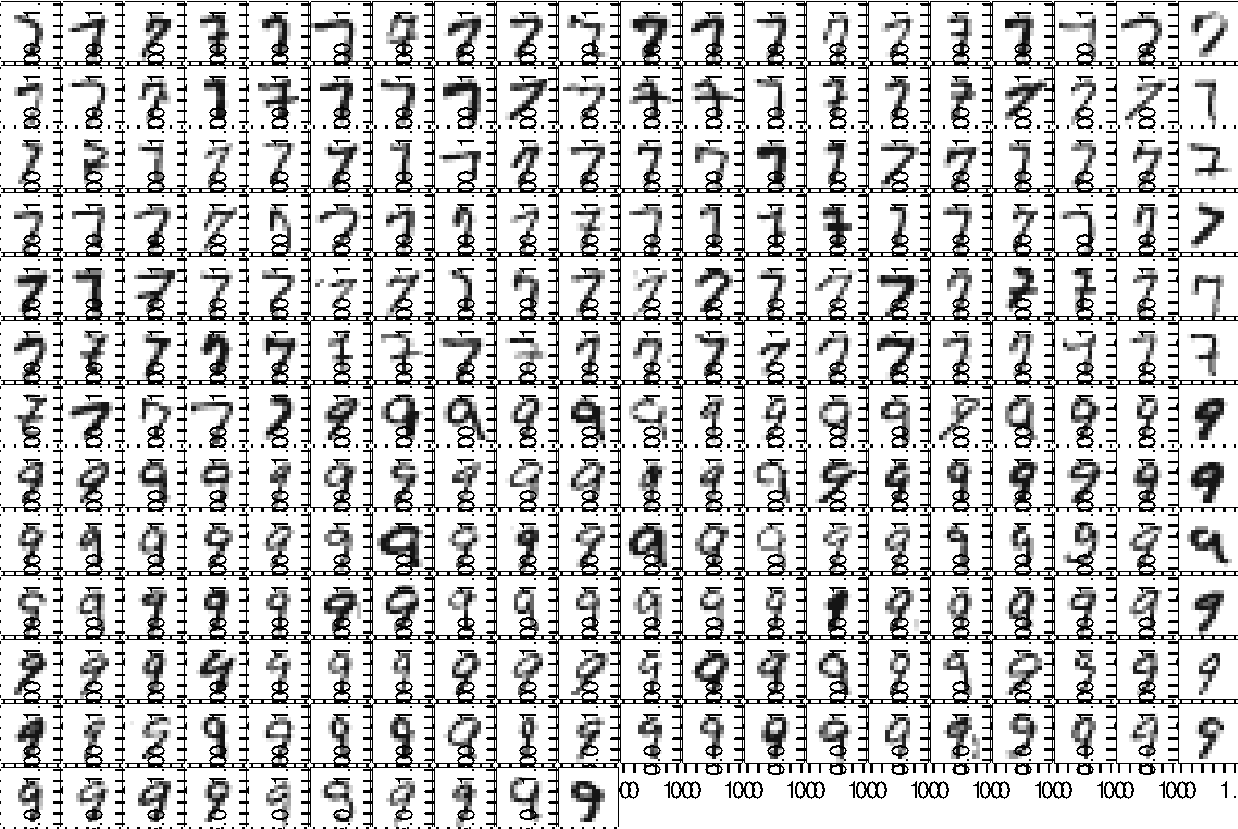
\includegraphics[width=1\linewidth]{ch-al/figures/data.pdf}
		\caption[MNIST data used in the simulations.]{MNIST data used in the 
		simulations. The digits 7 and 9 are similar visually, making 
		the simulations more realistic as it is harder for the classification 
		model to achieve a ``perfect fit'' (given only the initial labeled) 
		without the use of querying.}
		\label{fig:al:simulations:data}
	\end{center}
\end{figure}

\subsection{Evaluation}
\label{sec:al:simulation:evaluation}
The performance of a learner at any given point in time (at any iteration 
\textit{i} of simulation number $k \in [1,25]$) is encapsulated in its error 
ratio $\epsilon$. That is, given the current labeled set, the \textbf{main 
classifier (Random Forest model)} is trained, and the entire dataset is 
predicted given the current classifier. The predictions are stored in an 
$n$-length vector $p$. 
We know the true labels ahead of time (thanks to the MNIST dataset), and they 
are stored in an $n$-length vector $y'$. The predictions are compared against 
the true labels and the error ratio of iteration $i$ is given by
$$\epsilon_i = \frac{1}{250} \bigg( \sum\limits_{z=1}^{250} 
\textbf{1}_{p_z \neq y'_z} \bigg)$$

\noindent where $\textbf{1}_{p_z \neq y'_z}$ is an indicator variable that is 1 
when $p_z \neq y'_z$ and 0 otherwise. These 50 error ratios then form one 
vector $\epsilon_s$, the result of trial 
$s$. To select the best active learning algorithm \textit{on average}, each 
algorithm's error ratios are averaged over 25 total trials. This helps offset 
the randomness of the initialization and pooling scheme. Then the final error 
ratio of an algorithm is given by
$$\epsilon = \frac{1}{25} \bigg( \sum\limits_{i=1}^{25} \epsilon_s \bigg)$$

The final framework for computing $\epsilon_s$, a single trial's vector of 
error ratios, is summarized as follows (This procedure is encapsulated by the 
simulation engine code in 
Appendix~\ref{sec:appendicies:al:simulations:simengine}):

\tablespacing
\begin{algorithm}[H]
	\caption{Computing $\epsilon_s$, a single trial's vector of error 
	ratios}\label{alg:al:simulation:evaluation}
	\begin{algorithmic}[1]
		\Procedure{}{$X$ is a $n\times d$ matrix of $d$ observations of all $n$ 
			variables, $y$ is an $n$-length vector of labels for each variable 
			in $X$ ($y_i$=N/A when $X_{i,}$ has no label). $y'$ is an 
			$n$-length vector of \textbf{true} labels for each variable in $X$. 
			$iter$ is the maximum number of queries allowed per trial}
		\State \textbf{loop from} $i=1$ \textbf{to} $iter$:
		\State \indent $idx \gets $ active\_learning\_method$(X,y,...)$
		\State \indent \textsc{Query} $X_{idx,}$
		\State \indent $tout \gets 
		\text{train}(X^{labeled},y^{labeled},\text{randomforest})$
		\State \indent $p \gets \text{predict}(tout,X)$
		\State \indent $res_i\gets \frac{\text{length}(\text{which}(p \neq y'))}
		{\text{length}(y')}$
		\State \textbf{return} $res$
		\EndProcedure
	\end{algorithmic}
\end{algorithm}
\bodyspacing

\subsection{Summary of methods}
\label{sec:al:simulation:methods}

Table~\ref{tab:al:simulations} contains a summary of the active learning 
methods used in the simulation with details such tuning parameter values. 
Random sampling is used as the active learning method's control as a point of 
comparison; it is the most simplistic base case in which active learning is not 
present.

\tablespacing
\begin{longtable}{p{0.15\linewidth} p{0.21\linewidth} p{0.18\linewidth} 
p{0.4\linewidth}}
	
	% First page heading
	\caption[Summary of simulation active learning methods.]{A summary of the  
	active learning methods tested in the simulation. *\textit{Note:} The 
	classification model is the main classification model that is used to fit 
	the error, not the classification model(s) used in the active learning 
	methods (those are parameters). 
	The classification model in the simulator is akin to the main 
	classification model in the VS.} 
	\label{tab:al:simulations}\\
	\toprule
	\textbf{AL method} & \textbf{Simulations} & 
	\textbf{Classification model*} & \textbf{Parameters} \\
	\midrule
	\endfirsthead
	
	% Future page heading
	\caption[]{(continued)}\\
	\toprule
	\textbf{AL method} & \textbf{Simulations} & \textbf{Main classification 
	model} & \textbf{Parameters} \\
	\midrule
	\endhead
	
	% Page footer
	\midrule
	\multicolumn{4}{r}{(Continued on next page)}\\
	\endfoot
	
	% Last page footer
	\bottomrule
	\endlastfoot
	
	Random \newline sampling \newline (CONTROL) & 
	25 trials, 50 iterations, 15 ``pooled'' points each & 
	Random forest & 
	\textit{Classifier}: None \\
	
	\cmidrule[0.1pt](l{0.5em}r{0.5em}){1-4}	
	
	Uncertainty \newline sampling ~\ref{sec:al:methods:uncertainty} & 
	25 trials, 50 iterations, 15 ``pooled'' points each & 
	Random forest & 
	\textit{Classifier}: Random forest \\

	\cmidrule[0.1pt](l{0.5em}r{0.5em}){1-4}
	
	Query by \newline committee ~\ref{sec:al:methods:qbc} & 
	25 trials, 50 iterations, 15 ``pooled'' points each & 
	Random forest &	
	\textit{Committee}: RF, NB, SVM, PLS, \newline 
	\textit{Disagreement}: Vote entropy, \newline 
	\textit{C\_Pruning}: T, $\epsilon$: 0.5 \\ & \\
	
	& & Majority \newline committee \newline vote &	
	\textit{Committee}: RF, NB, SVM, PLS, \newline 
	\textit{Disagreement}: Vote entropy, \newline 
	\textit{C\_Pruning}: T, $\epsilon$: 0.5 \\ & \\
	
	(QBC \newline CONTROL) & & Random forest &	
	\textit{Committee}: RF, NB, SVM, PLS, \newline 
	\textit{Disagreement}: Vote entropy, \newline 
	\textit{C\_Pruning}: F, $\epsilon$: N/A \\ & \\
	
	& & Majority \newline committee \newline vote &	
	\textit{Committee}: RF, NB, SVM, PLS, \newline 
	\textit{Disagreement}: Vote entropy, \newline 
	\textit{C\_Pruning}: F, $\epsilon$: N/A \\	
	
	\cmidrule[0.1pt](l{0.5em}r{0.5em}){1-4}	
	
	Query by \newline bagging ~\ref{sec:al:methods:bagging} & 
	25 trials, 50 iterations, 15 ``pooled'' points each & 
	Random forest &
	\textit{Classifier}: Random forest, \newline \textit{Disagreement}: Vote 
	entropy, \newline \textit{num\_class}: 5, \textit{r}: 0.75 \\
		
	\cmidrule[0.1pt](l{0.5em}r{0.5em}){1-4}	
	
	Min-max \newline clustering ~\ref{sec:al:methods:clustering} & 
	25 trials, 50 iterations, 15 ``pooled'' points each & 
	Random forest & 
	\textit{Classifier}: None, \newline \textit{Distance}: Euclidean \\
	
\end{longtable}
\bodyspacing

\noindent QBC was tested with different parameters for the overall/main 
classification model (random forest vs majority committee vote) and committee 
pruning (yes or no). This was done in order to see the effectiveness of the 
proposed addendums to the QBC method (Section~\ref{sec:al:methods:qbc}) and, 
ultimately, select the best QBC method in terms of \textit{algorithm structure} 
for comparison with the other methods. Naturally, the control for comparing the 
QBC methods is the method with a random forest classification model and no 
committee pruning (This turns into the naive QBC methodology as detailed in 
Algorithm~\ref{alg:al:methods:qbc1}). A general committee was randomly selected 
which worked with the data. For example, any form of discriminant analysis, 
which utilizes matrix inversion, does not work without data cleaning. The 
nature of the MNIST data is that many columns are 0 (white space). This is 
evident from the plots in Figure~\ref{fig:al:simulations:data}. These columns 
of 0 makes the matrix degenerate, so discriminant analysis cannot function. 
To avoid further tampering with the dataset (as the data has already been 
compressed), LDA, DDA, FDA, etc. were not included in the starting committee. 
A summary of each classification model used in the starting committee for QBC 
implementation is as follows:

\tablespacing
\begin{itemize}
	\item \textbf{Random Forest:} A random forest is a collection of decision 
	trees which are grown from independent draws of the training set. A more 
	detailed description can be found in 
	Section~\ref{sec:visualizer:plotgeneration:tree}.
	\item \textbf{Naive Bayes:}
	\item \textbf{SVM:}
	\item \textbf{Partial Least Squares:}
\end{itemize}
\bodyspacing

The call to each active learning function is controlled by the AL engine code 
in Appendix~\ref{sec:appendicies:al:simulations:alengine}. By implementing the 
active learning call in this way, the main AL functions are hidden from the end 
user so that they cannot call the functions directly, which may lead to 
bypassing checks and/or improperly calling functions.



\subsection{Results}
\label{sec:al:simulation:results}

The full simulator which loads the data (using functions in 
Appendix~\ref{sec:appendicies:al:simulations:data}), calls the simulation 
engine (Appendix~\ref{sec:appendicies:al:simulations:simengine}) 25 times for 
each active learning method (the simulation engine calls the active learning 
engine, Appendix~\ref{sec:appendicies:al:simulations:alengine}), and averages 
then plots the results may be found in 
Appendix~\ref{sec:appendicies:al:simulations:results}.

\begin{figure}[htb]
	\begin{center}
		\includegraphics[width=1\linewidth,page=2]{ch-al/figures/results.pdf}
		\caption[Active learning simulation results for Query by Committee with 
		varying parameters.]{Active learning simulation results for Query by 
			Committee with varying parameters. Each of the 25 trials were 
			consistently seeded with its own value, so the values before 
			committee pruning would/would not have occurred (at $iter/2=25$) 
			are the same. }
		\label{fig:al:simulations:resultsqbc}
	\end{center}
\end{figure}

Figure~\ref{fig:al:simulations:resultsqbc} is a summarization of the 
performance of query by committee given different parameters. With query by 
committee, majority committee vote outperforms random forest on 
average in the first half (25 iterations) as the main classification model. 
What is interesting to note in iteration 25 onwards is that the error ratio for 
both majority committee vote spikes up \textit{after pruning has occurred}. 
This is interesting since the idea was to prune committee who performed poorly; 
this indicates that the insight of \textit{all} committee members, 
despite performance (or with more room for error than 0.5), are valuable. 
Naturally, this phenomenon cannot be observed in the random forest results 
because the classification model is a random forest; since committee members 
are not weighing in on the predicted labels, the members themselves hold 
less weight. Although majority committee voting with no pruning 
continues to maintain its lead past 25 iterations, the error ratios converge as 
the number of iterations gets closer to 50. In fact, near iteration 50, it 
appears that both random forest methods start converging faster and just barely 
overtake majority committee vote at the end. In other words, QBC with majority 
voting starts off better but improves more slowly while QBC with random foresst 
starts off worse but improves more rapidly.
Each method has its own trade-offs, and it becomes all the more important to 
keep the end goal, the visualization system, in mind. Recall that an important 
criterion for active learning performance is performance given {less query
points}. The user should not have to label more than fifty plots in order for 
the system to learn his/her interests; not only is it tedious for the user, but 
this tedium may cause the user to perform the tasks with less seriousness or 
cause the user's concentration to slip. Subsequently, we select \textbf{QBC 
with majority committee vote and no committee pruning} for comparison with the 
other algorithm types.

\begin{figure}[htb]
	\begin{center}
		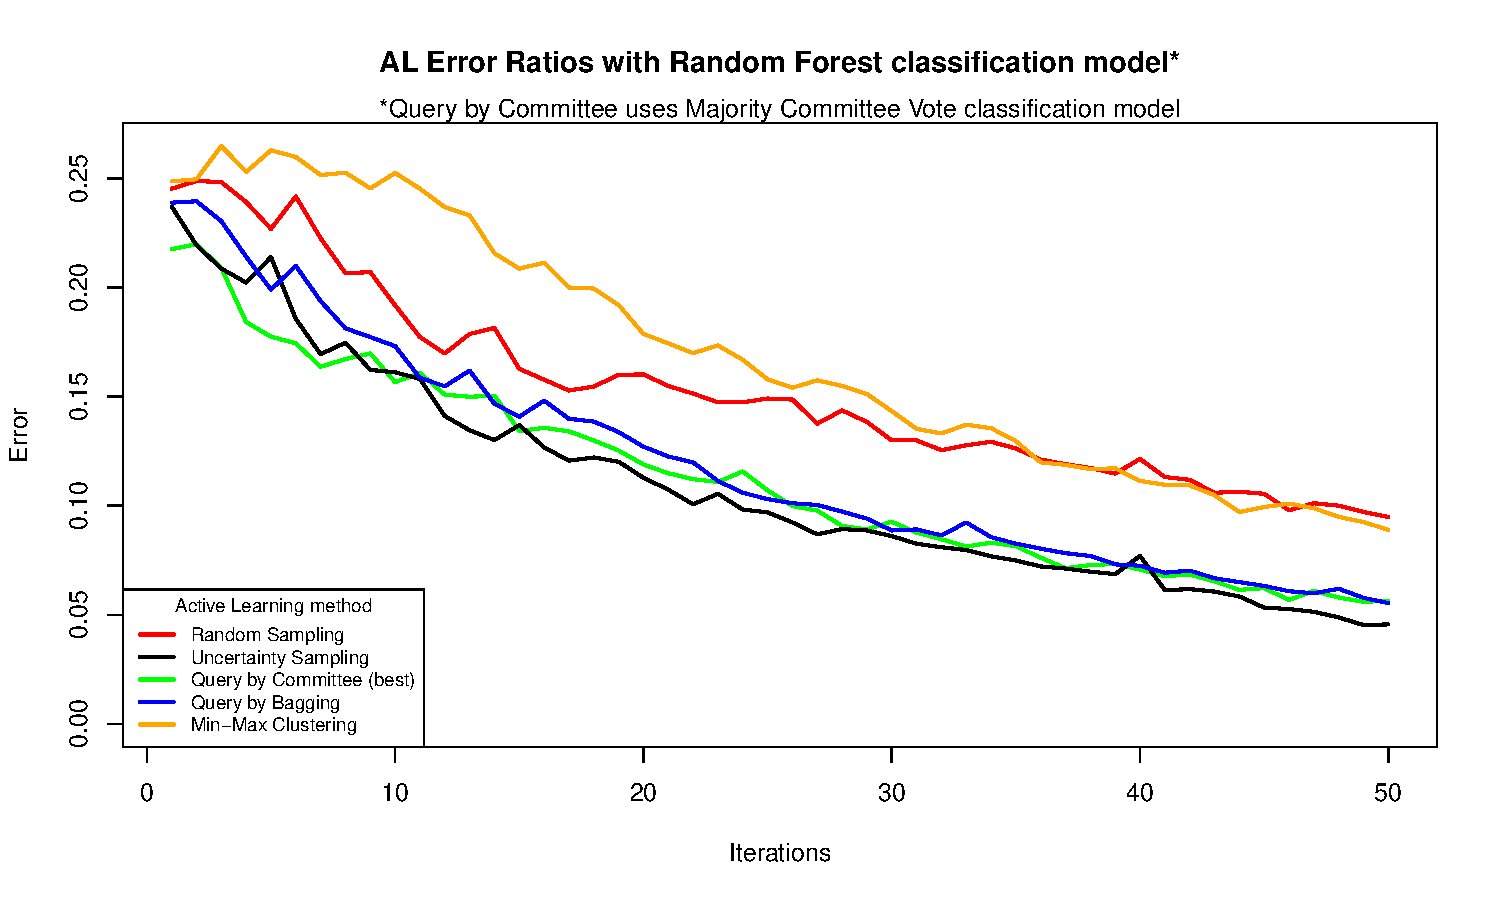
\includegraphics[width=1\linewidth,page=1]{ch-al/figures/results.pdf}
		\caption[Aggregated active learning simulation results.]{ 
		Aggregated active learning simulation results.}
		\label{fig:al:simulations:results}
	\end{center}
\end{figure}

Figure~\ref{fig:al:simulations:results} summarizes the performance of the 
``best'' QBC method against the other active learning methods along with random 
sampling as a control (a baseline for comparisons). Random sampling actually 
performs better than one might expect, though it is the first to fall off 
(converge more slowly). This may be, in part, due to the constraints of 
pool-based sampling. In each iteration, random sampling was also constrained to 
15 random points each to query from. Thus, each active learning method cannot 
optimize over the entire sample space.

What is especially interesting is that random 
sampling performs better than min-max clustering for the longest time (but 
min-max clustering converges more rapidly and eventually overtakes random 
sampling). This may be attributed to the nature of the active learner's 
initialization. With clustering algorithms, initialization is extremely 
important; by starting with points within clusters, the min-max methodology 
allows the learner to further query within clusters (to sample more labels) 
without having to start by searching through the entire space for the clusters. 
In the simulator, recall that each active learning method is initialized 
randomly with the same set of data and starting points. We suspect that if we 
had initialized the min-max clustering method with the $k$-nearest neighbors 
graph as suggested by Vu \textit{et al.}  ~\cite{vu2010}, the min-max 
clustering algorithm would have begun with better performance. 

Query by bagging, overall, performs worse than query by committee. In fact, it 
performs similarly to QBC with a main random forest classification model, whose 
performance can be seen in Figure~\ref{fig:al:simulations:resultsqbc}. 
This isn't surprising because the bagging algorithm itself uses a committee of 
five random forest classifiers (these parameters are summarized in 
Table~\ref{tab:al:simulations}) and also uses a random forest 
for the main classification model. 

There appears to be another ``tie'' for query by committee and uncertainty 
sampling. QBC starts off better, but the faster convergence in uncertainty 
sampling eventually outperforms QBC. Unlike the case of QBC with a random 
forest versus majority committee vote classification model 
(Figure~\ref{fig:al:simulations:resultsqbc}), uncertaintly sampling overtakes 
QBC much earlier. To be more specific, QBC is overtaken near the tenth 
iteration. Thus, out of all methods described in 
Table~\ref{tab:al:simulations}, \textbf{uncertainty sampling} most closely 
embodies the qualities that characterize a strong active learner: intelligent 
selection of queries that allow the main classifier to learn interests more 
quickly.

Figure~\ref{fig:al:simulations:resultsci}, which shows performance plots with 
confidence intervals for each active learrning method, may also be of interest 
to the reader.

%\textsc{\begin{figure}[htb]
%	\begin{center}
%		\includegraphics[width=1\linewidth,page=3]{ch-al/figures/results.pdf}
%		\caption[Active learning simulation results with confidence 
%		intervals.]{Active learning simulation results with confidence 
%		intervals.}
%		\label{fig:al:simulations:resultsci}
%	\end{center}
%\end{figure}}

\subsubsection{Extensions}

Naturally, there are many other parameters that could have been tested, which 
were not tested in this simulator in the interest of time. For 
example, the classification model in the active learning method (not the 
overall method) to aid in query selection does not have to be a random forest 
(This applies to US and QBB); perhaps another would have worked better despite 
the intuition that, if the active learning methods optimizes over the same 
classification model that the main program will use, the learner will perform 
better. As noted earlier, initialization is important for min-max clustering, 
and the performance of the learner may be tested with different initialization 
schemes. Furthermore, there are other disagreement methods 
that could be implemented aside from vote entropy, one of which was described 
earlier in Section~\ref{sec:al:methods:qbc} (This applies to QBC and QBB). The 
tuning parameters of $\epsilon$ and $r$ in the query by committee/bagging 
methods could also be perturbed to see the effect on error ratio. Finally, 
different committees could be fed into the QBC method, and different starting 
points for pruning (i.e. $iter/3$ or $iter/4$ instead of $iter/2$) could also 
be tested. It may also be of interest to dig into why the active learner 
suddenly does worse the moment a committee is pruned. The reader is invited to 
pursue these as further extensions of this work should they wish to.